\documentclass{beamer}
\usetheme[compress]{Padova}
\usepackage{presentazione}
\usepackage{tikz}
\usetikzlibrary{arrows}
\addbibresource{msbd.bib}
\title{\textsc{Classificazione di attività motorie tramite accelerometro del cellulare}}
\author{Luisa Galtarossa\and Alberto Grassi\and Anna Montin\and Daniele Zago}
\date{}
\newcommand{\getsection}{\color{white}\insertsection}

\begin{document}
\begin{frame}
\titlepage
\end{frame}

\section{Introduzione}
\begin{frame}{Il problema analizzato}
Ormai con il cellulare è possibile fare moltissime cose. 
Cancellare messaggi, avere più giga\dots È tutto possibile con un solo shake.\\
\smallskip
\textbf{Ma come si può riconoscere uno shake?}
\medskip
\begin{figure}[H]

\includegraphics[width=0.4\textwidth]{./images/vodafoneshake.png}
\end{figure}
\end{frame}

\begin{frame}{La nostra idea}
Riconoscere uno shake tra diverse attività motorie.\\
\smallskip
\begin{columns}[T] % align columns
\begin{column}{.48\textwidth}
Le attività analizzate sono:
\begin{itemize}
\item Camminata
\item Camminata con cellulare in tasca
\item Corsa
\item Corsa con cellulare in tasca
\item Utilizzo a riposo
\item Salti
\item Salita e discesa di scale
\item Shake
\end{itemize}
\end{column}%
\hfill%
\begin{column}{.4\textwidth}
\begin{figure}[H]
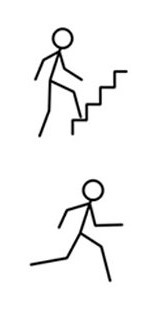
\includegraphics[width=0.6\textwidth]{./images/attivit.jpg}
\end{figure}
\end{column}%
\end{columns}
\end{frame}

\begin{frame}{L'accelerometro}
\begin{figure}[H]
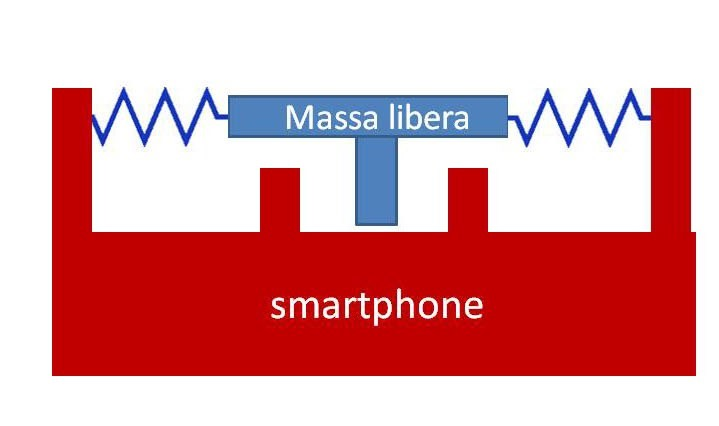
\includegraphics[width=0.55\textwidth]{../figure/accelerometro1.jpg}
\end{figure}
\begin{figure}[H]
\hspace{10pt}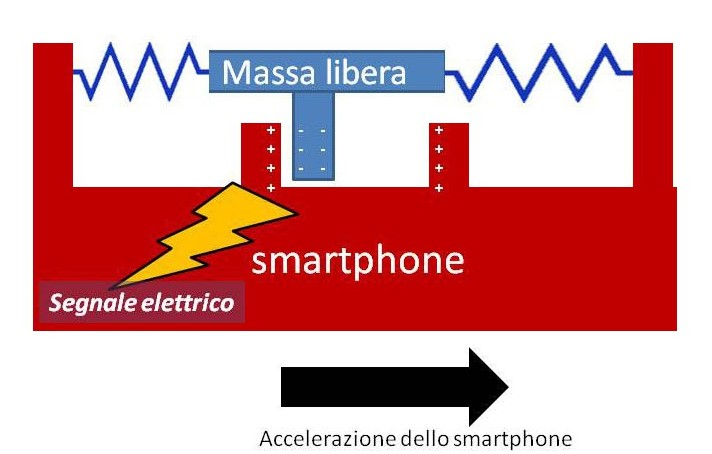
\includegraphics[width=0.55\textwidth]{../figure/accelerometro2.jpg}
\end{figure}
\end{frame}

\begin{frame}{Raccolta dati}
I dati sono stati raccolti tramite l'applicazione \texttt{PhonePi} \cite{kumarPhonePiSampleServer2019}.\\
\smallskip
Questa fornisce l'accelerazione $\vec{a}_t = \begin{pmatrix}a_{xt} \\ a_{yt} \\ a_{zt}\end{pmatrix}$ ad intervalli di $\SI{10}{ms}$.
\pause
\begin{figure}[H]
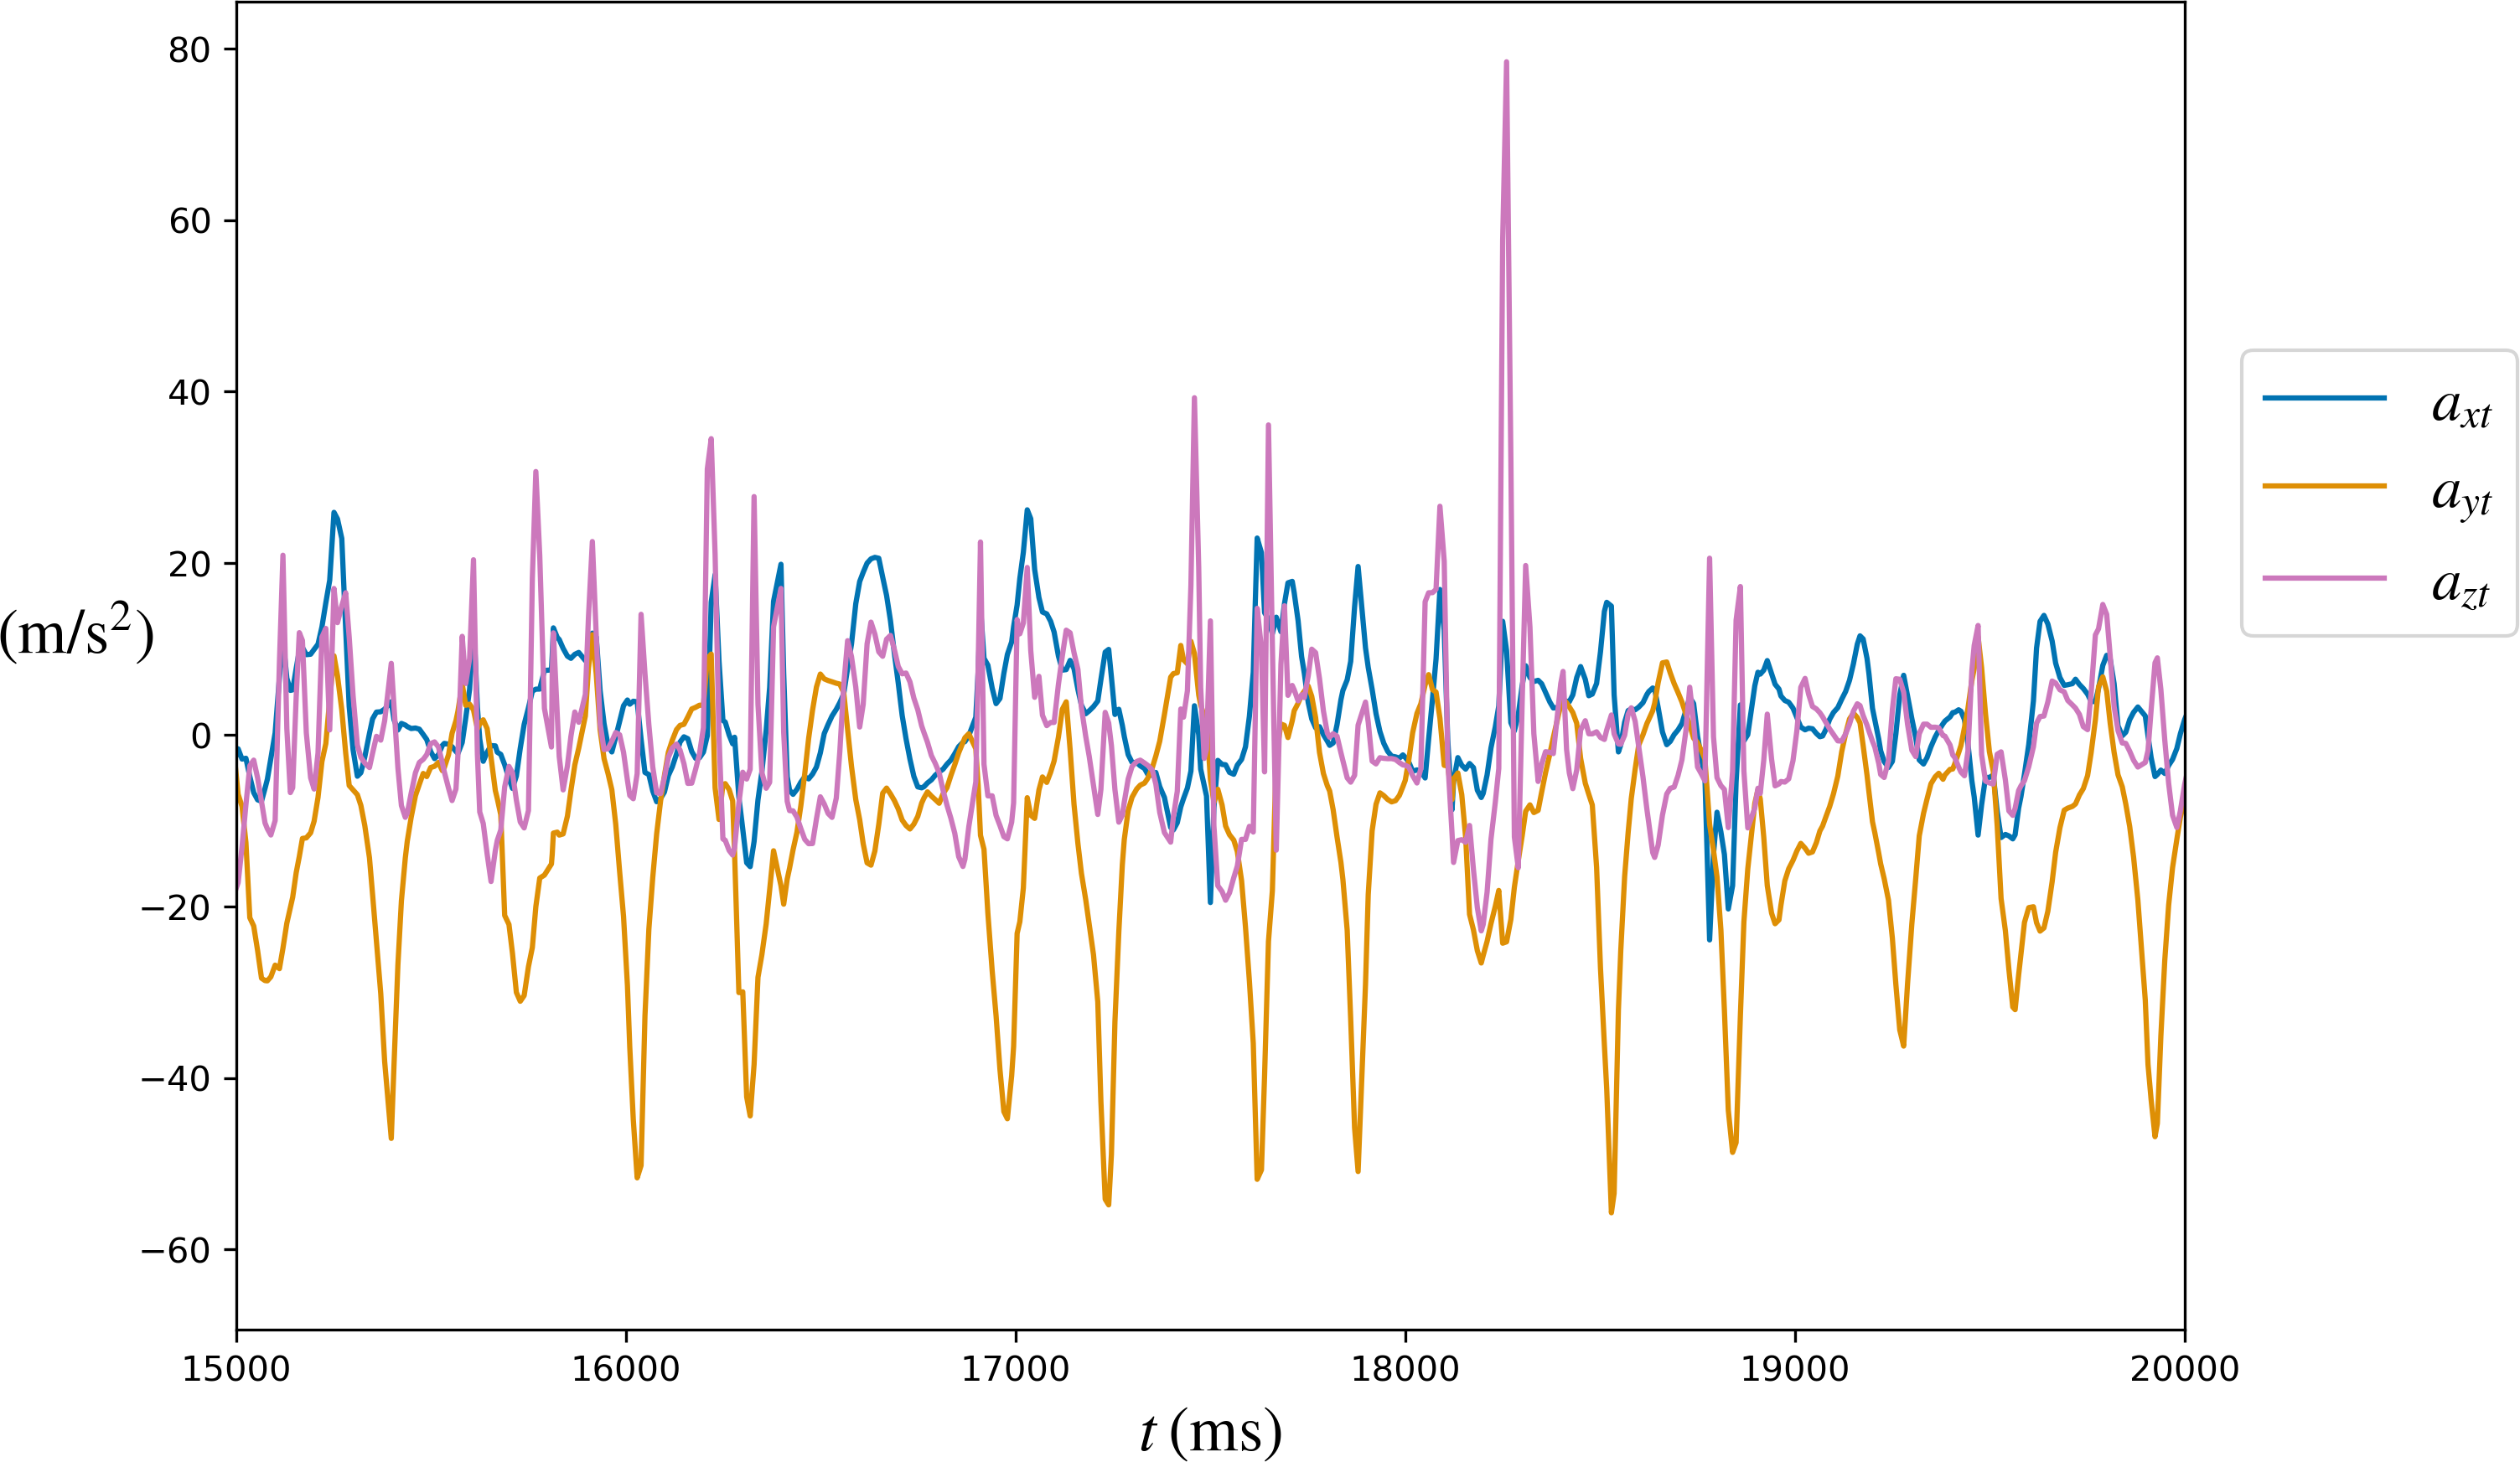
\includegraphics[width=0.85\textwidth]{../figure/esempio-accel.png}
\end{figure}
\end{frame}

\begin{frame}{Accelerazione} % conlusione magari come possibili miglioramenti --> 9.8 
Il sistema di riferimento dell'accelerometro è rotante, quindi $\vec{a}_t$ è difficile da trattare.
\begin{figure}[H]
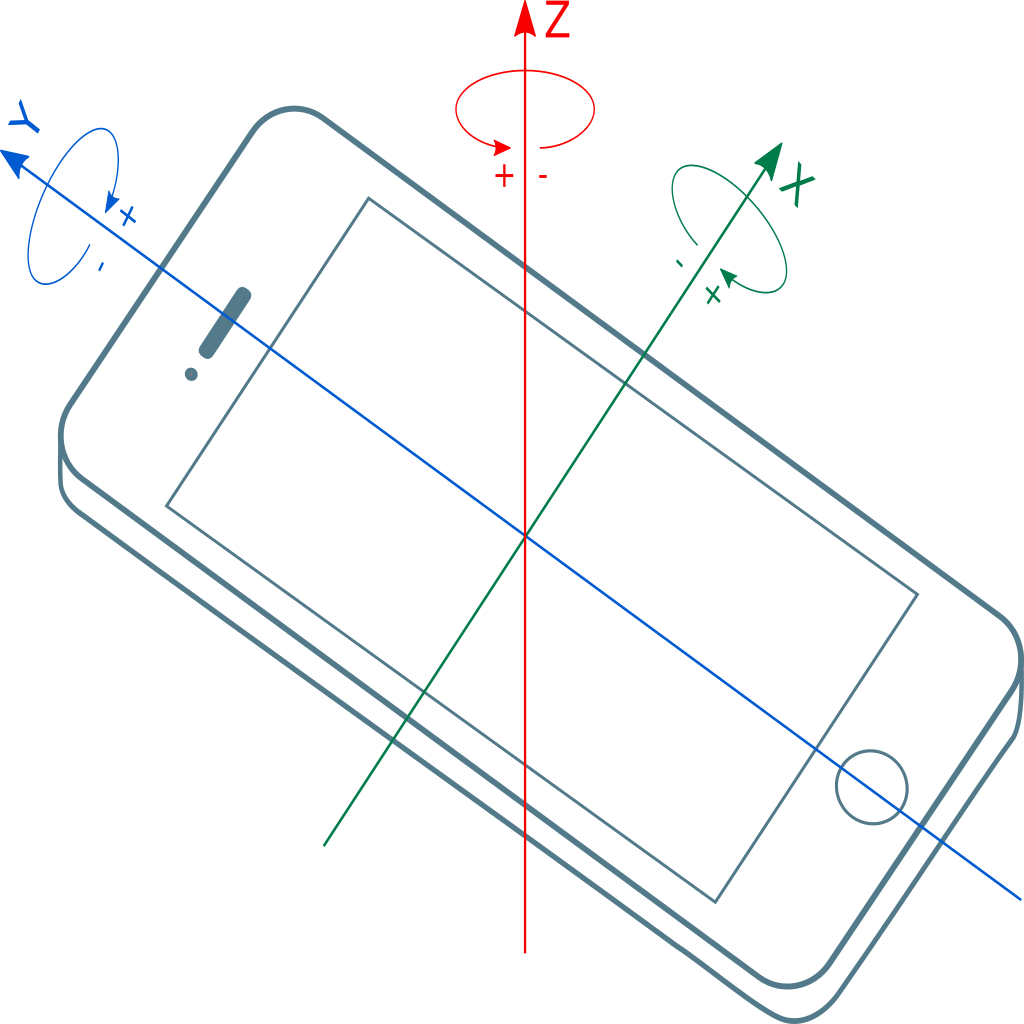
\includegraphics[width=0.6\textwidth]{../figure/sensor_coordinate_system.png}
\end{figure}

\end{frame}
\begin{frame}{Accelerazione}
Lavoriamo sul modulo dell'accelerazione $\|\vec{a_t}\| =\sqrt{a_{xt}^2+a_{yt}^2+a_{zt}^2}$.
\pause
\begin{figure}[H]
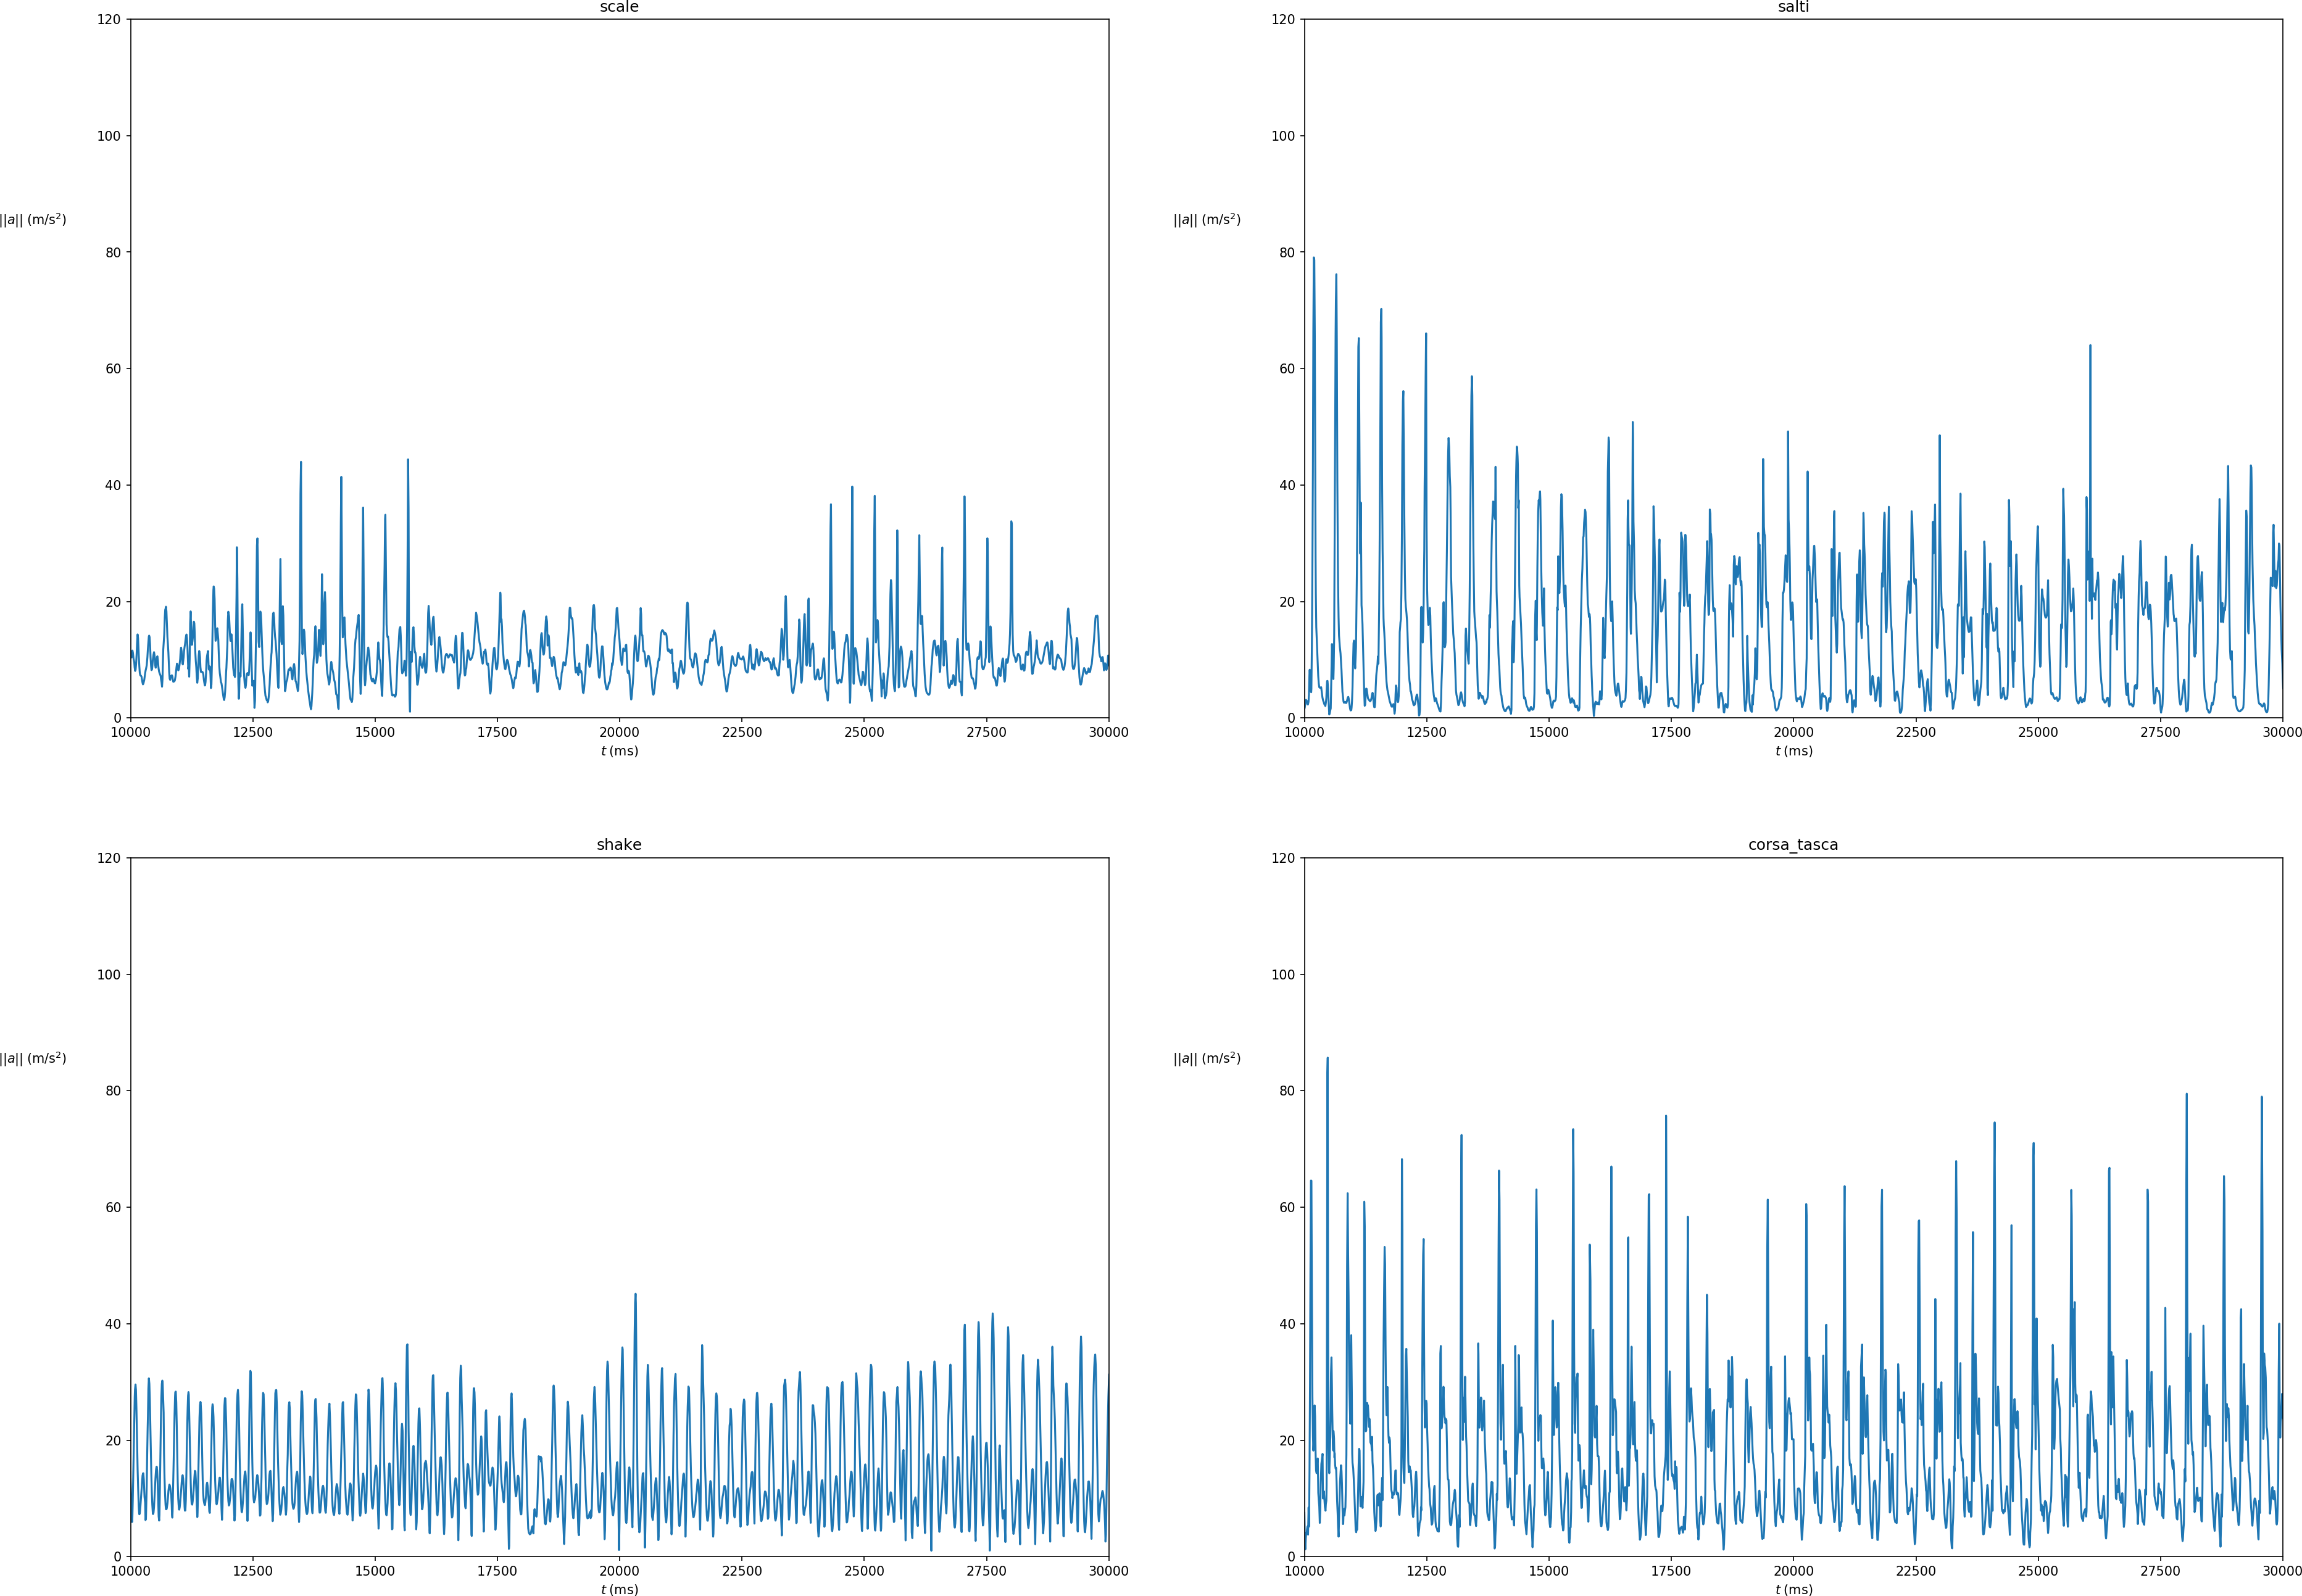
\includegraphics[width=0.85\textwidth]{../figure/espl.png}
\end{figure}
\end{frame}

\section{Esplorativa}
\begin{frame}{Accelerazione}
I dati sono stati suddivisi in intervalli di ampiezza $\SI{1.5}{s}$
\begin{table}[H]
\begin{tabular}{cccccccc}
\toprule
y & $\|\vec{a}_0\|$ & $\|\vec{a}_1\|$ & $\|\vec{a}_2\|$  & $\dots$ & $\|\vec{a}_{149}\|$\\
\midrule
camminata & 5.449 & 5.300 & 5.344 &  $\cdots$ & 13.147\\
camminata & 13.977 & 14.910 & 15.567 &  $\cdots$ & 5.480\\
camminata & 5.608 & 5.868 & 6.143 &  $\cdots$ & 18.227\\
camminata & 19.026 & 18.886 & 18.098 &  $\cdots$ & 6.299\\
$\vdots$ & $\vdots$ & $\vdots$ & $\vdots$ &  $\vdots$ & $\vdots$\\
shake & 11.480 & 14.663 & 16.968 &  $\cdots$ & 8.474\\
\bottomrule
\end{tabular}
\end{table}
\begin{center}
\pause \textbf{Perché non lavorare direttamente con le esplicative $\|\vec{a}_0\|,\dots,\|\vec{a}_{149}\|$?}
% il legame tra le accelerazioni è nessuno --> per quato usiamo le  esplicative 
\end{center}
\end{frame}


\begin{frame}{Le esplicative}
\begin{figure}[H]
	\centering
	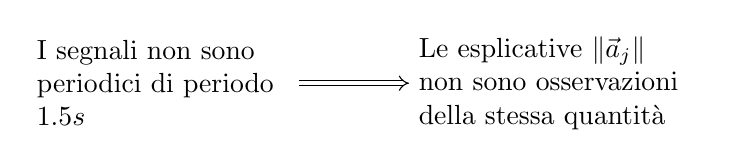
\begin{tikzpicture}
	\node[text width=3.2cm, align=left, rectangle] (a) at (-2.5,0){I segnali non sono periodici di periodo $\SI{1.5}{s}$};
	\node[text width=3.5cm, align=left	, rectangle] (b) at (2.5,0){Le esplicative $\|\vec{a}_j\|$ non sono osservazioni della stessa quantità};
	\draw[-implies,double equal sign distance] (a) -- (b);
	\end{tikzpicture}
\end{figure}
\pause
\begin{columns}[T] % align columns
\begin{column}{.49\textwidth}
\begin{figure}[H]
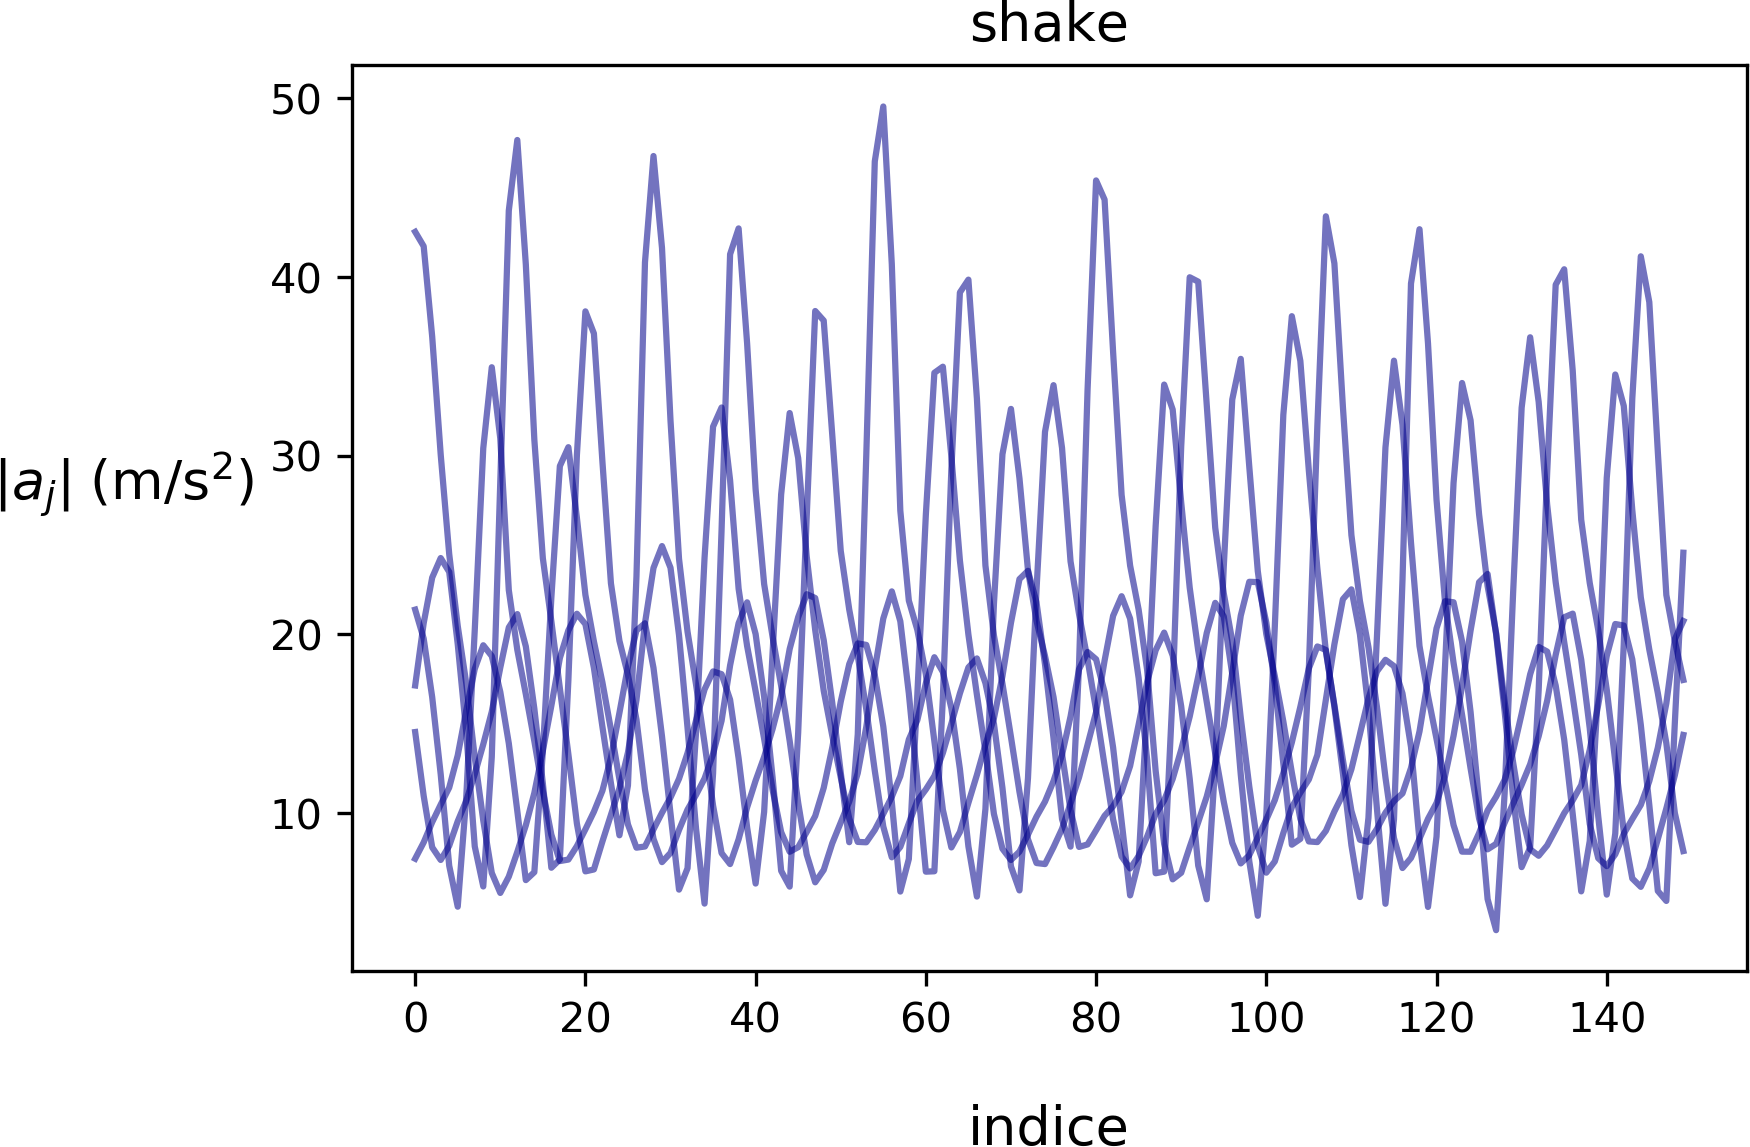
\includegraphics[width=.99\textwidth]{../figure/shake.png}
\end{figure}
\end{column}%
\hfill%
\begin{column}{.49\textwidth}
\begin{figure}[H]
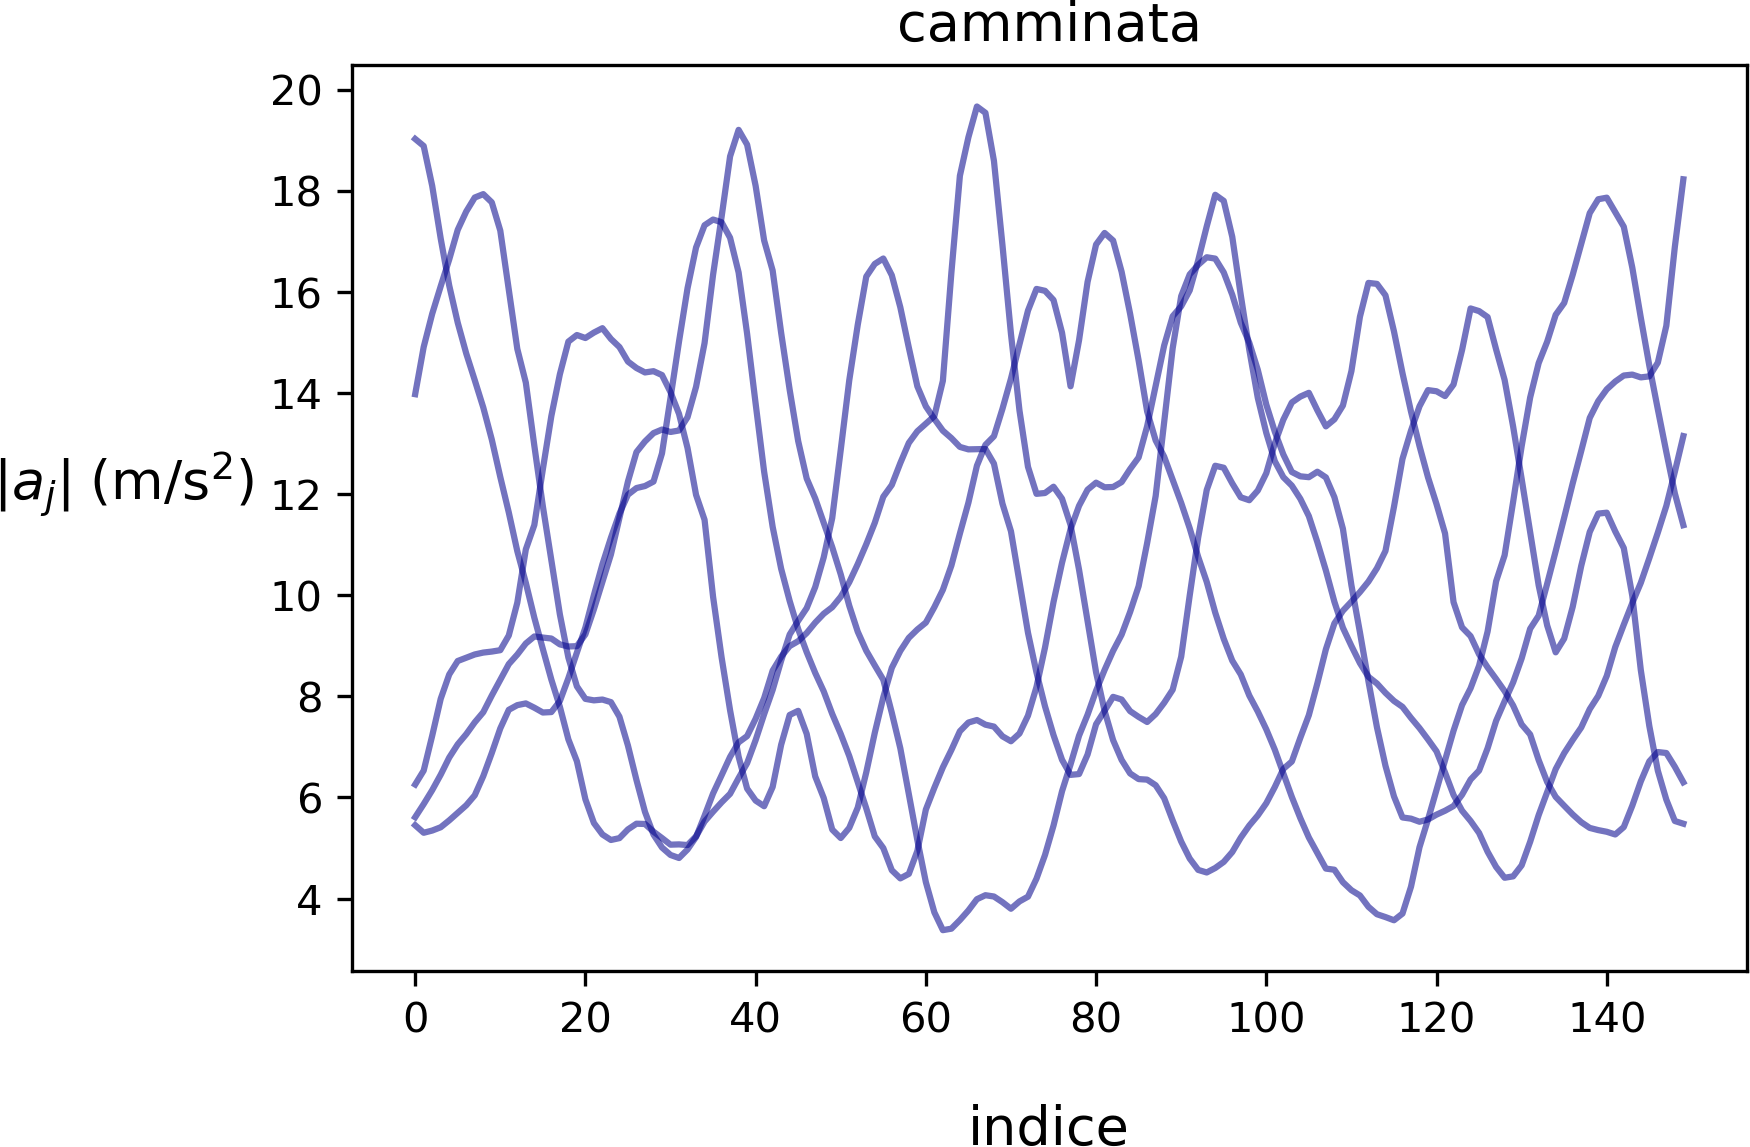
\includegraphics[width=.99\textwidth]{../figure/camminata.png}
\end{figure}
\end{column}%
\end{columns}
\end{frame}

\begin{frame}{Le esplicative}
\textbf{Soluzione}: usare indici riassuntivi dell'intervallo.
\begin{table}[H]
	\centering
	\begin{tabular}{ll}
		\texttt{minA}& Minimo dell'accelerazione.\\
		\texttt{medA}& Mediana dell'accelerazione.\\
		\texttt{varA}& Varianza dell'accelerazione.\\
		\texttt{maxA}& Massimo dell'accelerazione.\\
		\texttt{meanA}& Media dell'accelerazione.\\
		\texttt{MVDeriv}& Media del valore assoluto della derivata seconda.
	\end{tabular}
\end{table}
\end{frame}

\begin{frame}{\texttt{MVDeriv}}
\texttt{MVDeriv} serve per discriminare le alte frequenze dalle basse frequenze.\\
\bigskip
L'operazione di derivazione all'istante $t$ è approssimata con\cite{NumpyGradientNumPy}
\[
\dot{a}_t = \dfrac{a_{t + 1} - a_{t - 1}}{2}\,.
\]
\end{frame}

\begin{frame}{Analisi esplorative}
\begin{columns}[T] % align columns
\begin{column}{.33\textwidth}
\begin{figure}[H]
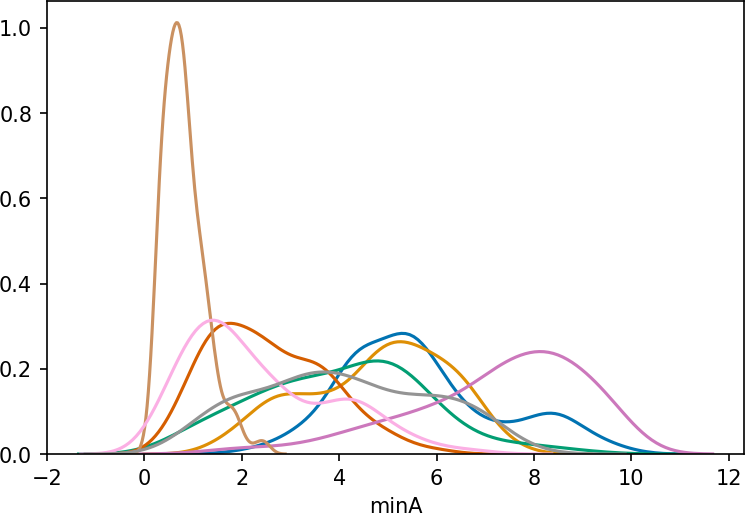
\includegraphics[width=\textwidth]{../figure/minA.png}
\end{figure}
\begin{figure}[H]
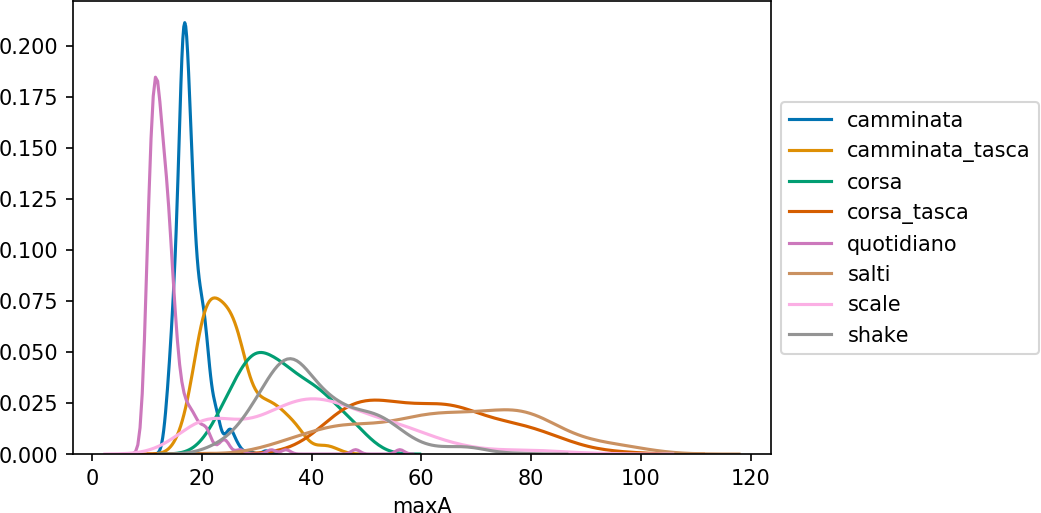
\includegraphics[width=\textwidth]{../figure/maxA.png}
\end{figure}
\end{column}%
\hfill%
\begin{column}{.33\textwidth}
\begin{figure}[H]
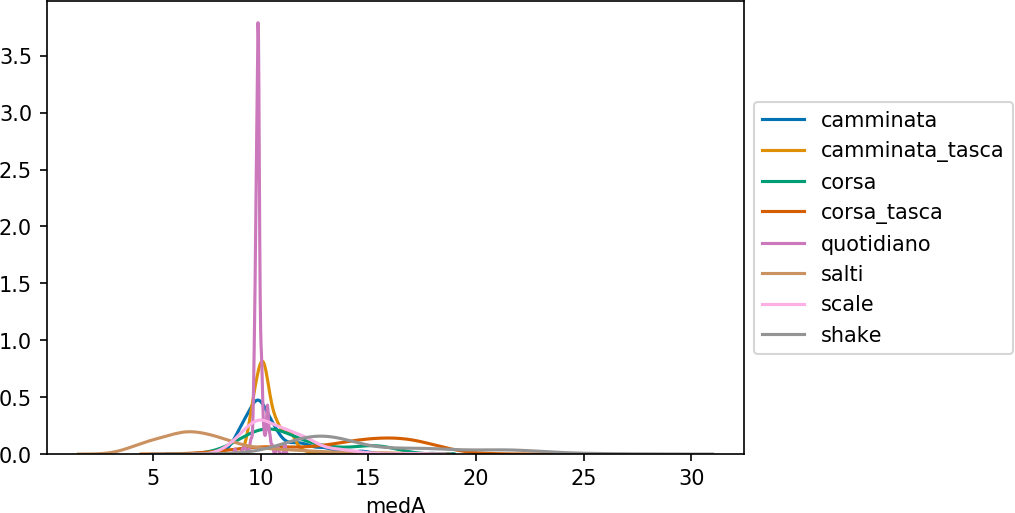
\includegraphics[width=\textwidth]{../figure/medA.png}
\end{figure}
\begin{figure}[H]
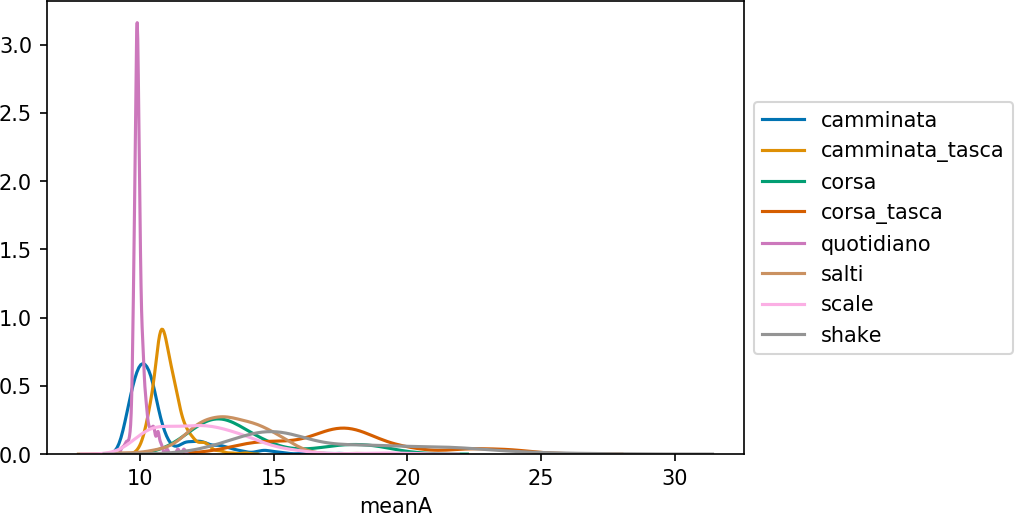
\includegraphics[width=\textwidth]{../figure/meanA.png}
\end{figure}
\end{column}%
\hfill%
\begin{column}{.33\textwidth}
\begin{figure}[H]
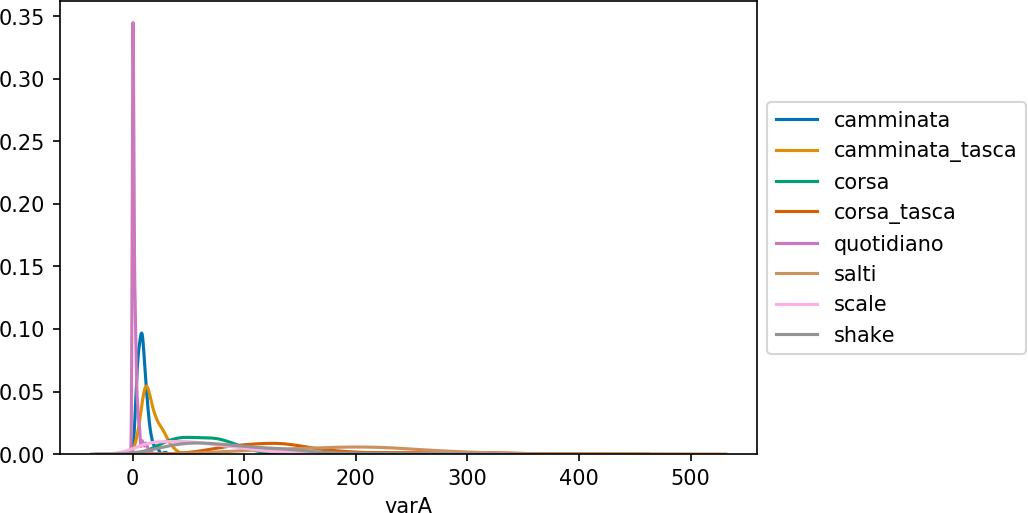
\includegraphics[width=\textwidth]{../figure/varA.png}
\end{figure}
\begin{figure}[H]
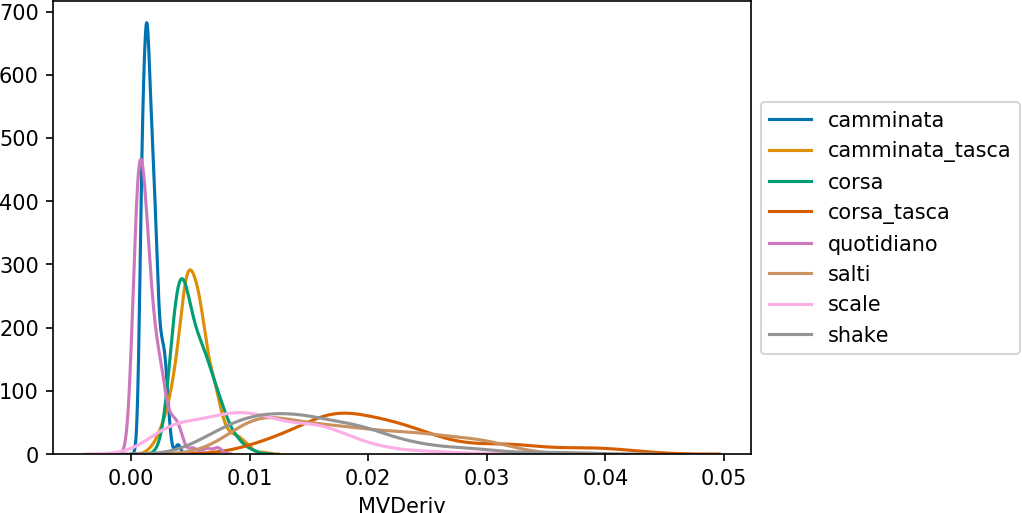
\includegraphics[width=\textwidth]{../figure/MVDeriv.png}
\end{figure}
\end{column}%
\end{columns}
\end{frame}


\begin{frame}{Analisi esplorative}
\begin{figure}[H]
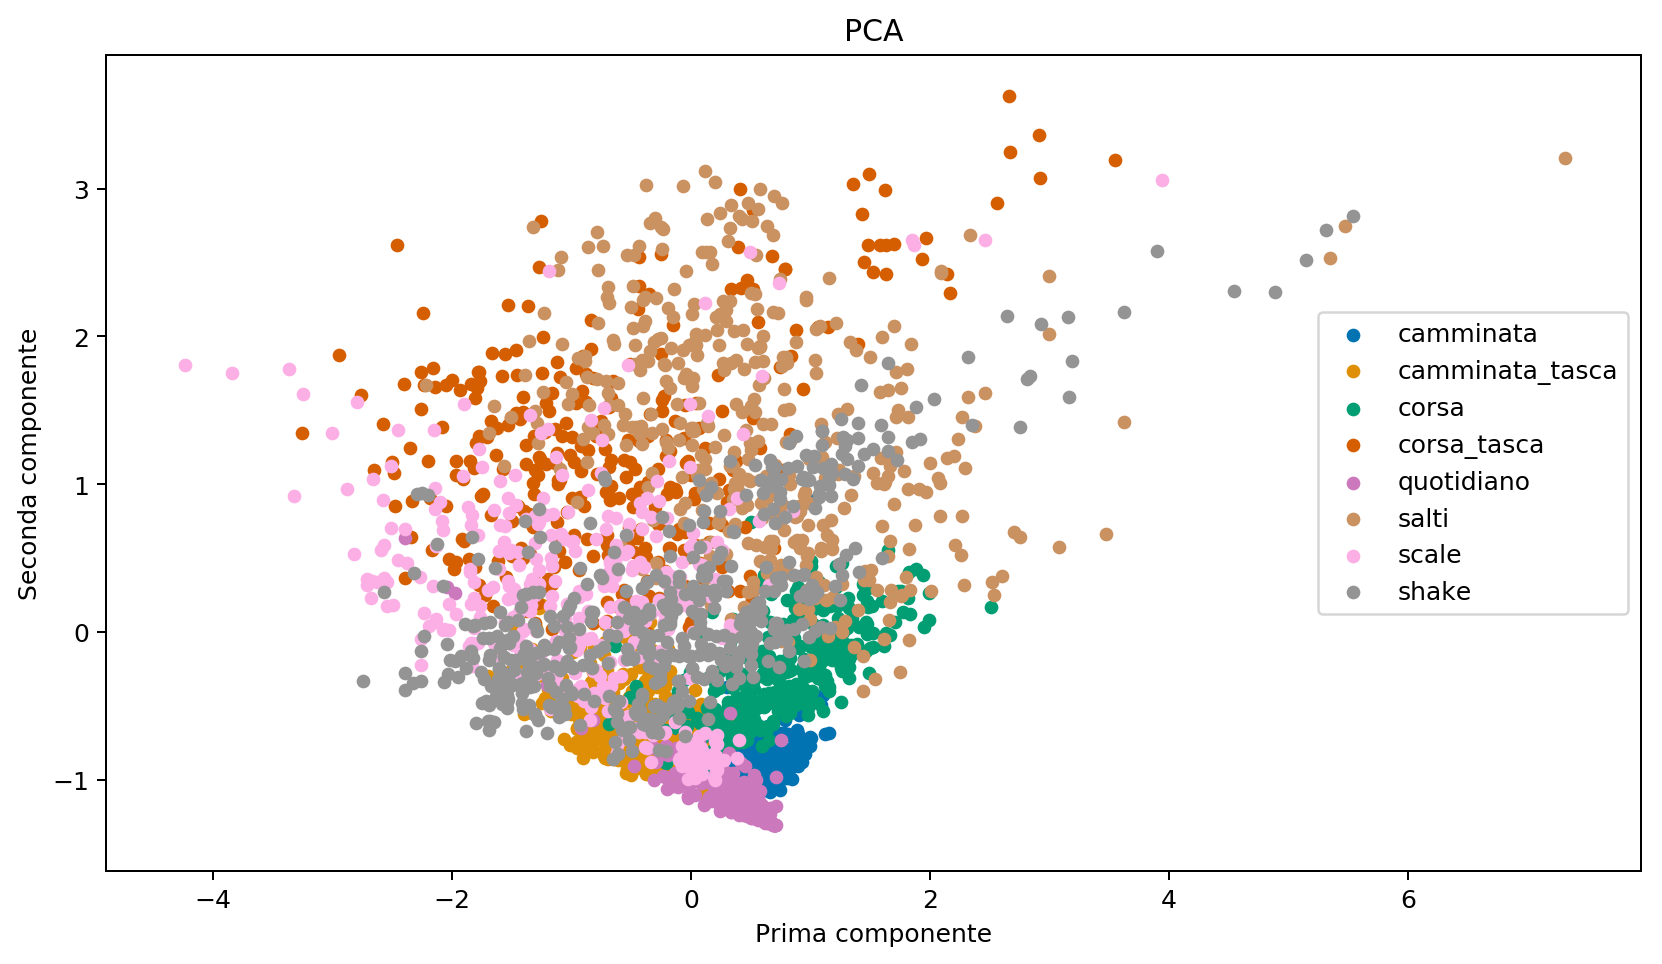
\includegraphics[width=0.7\textwidth]{../figure/PCA.png}
\end{figure}
\begin{figure}[H]
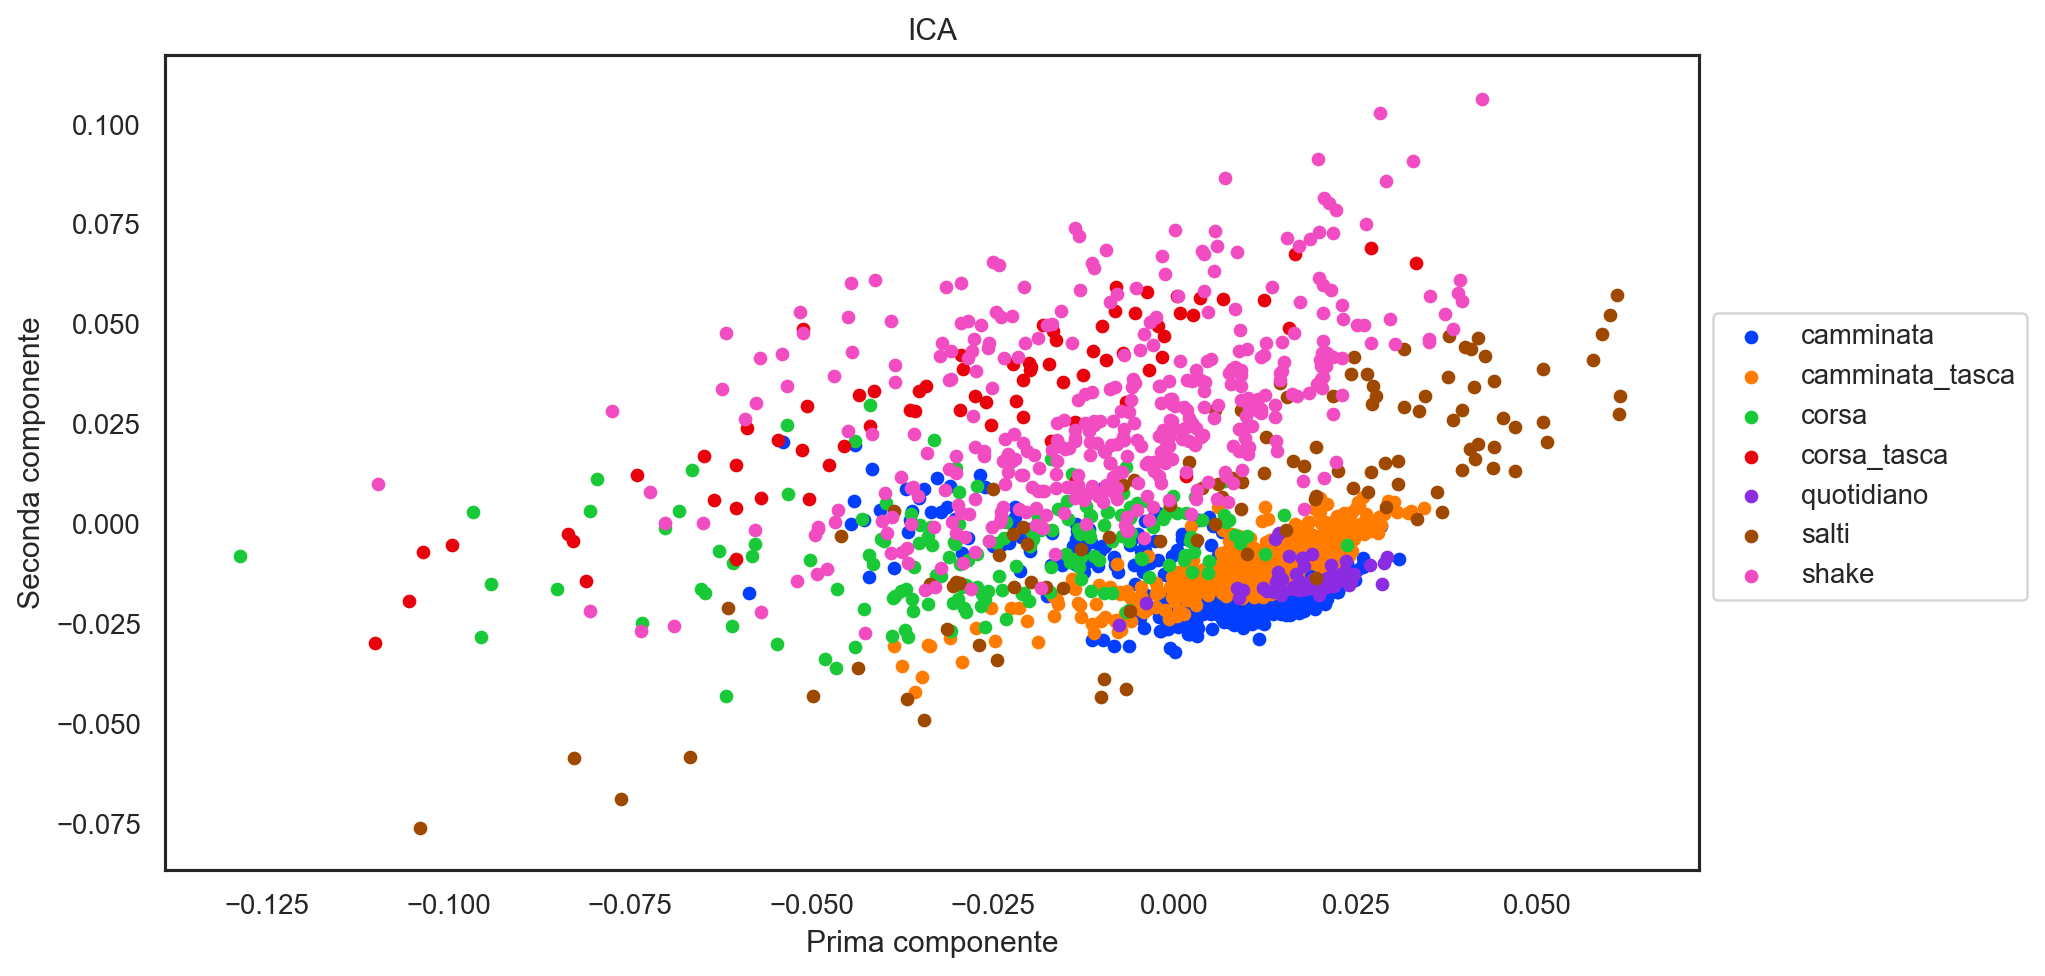
\includegraphics[width=0.7\textwidth]{../figure/ICA.png}
\end{figure}
\end{frame}

\begin{frame}{Analisi esplorative}
\begin{figure}[H]
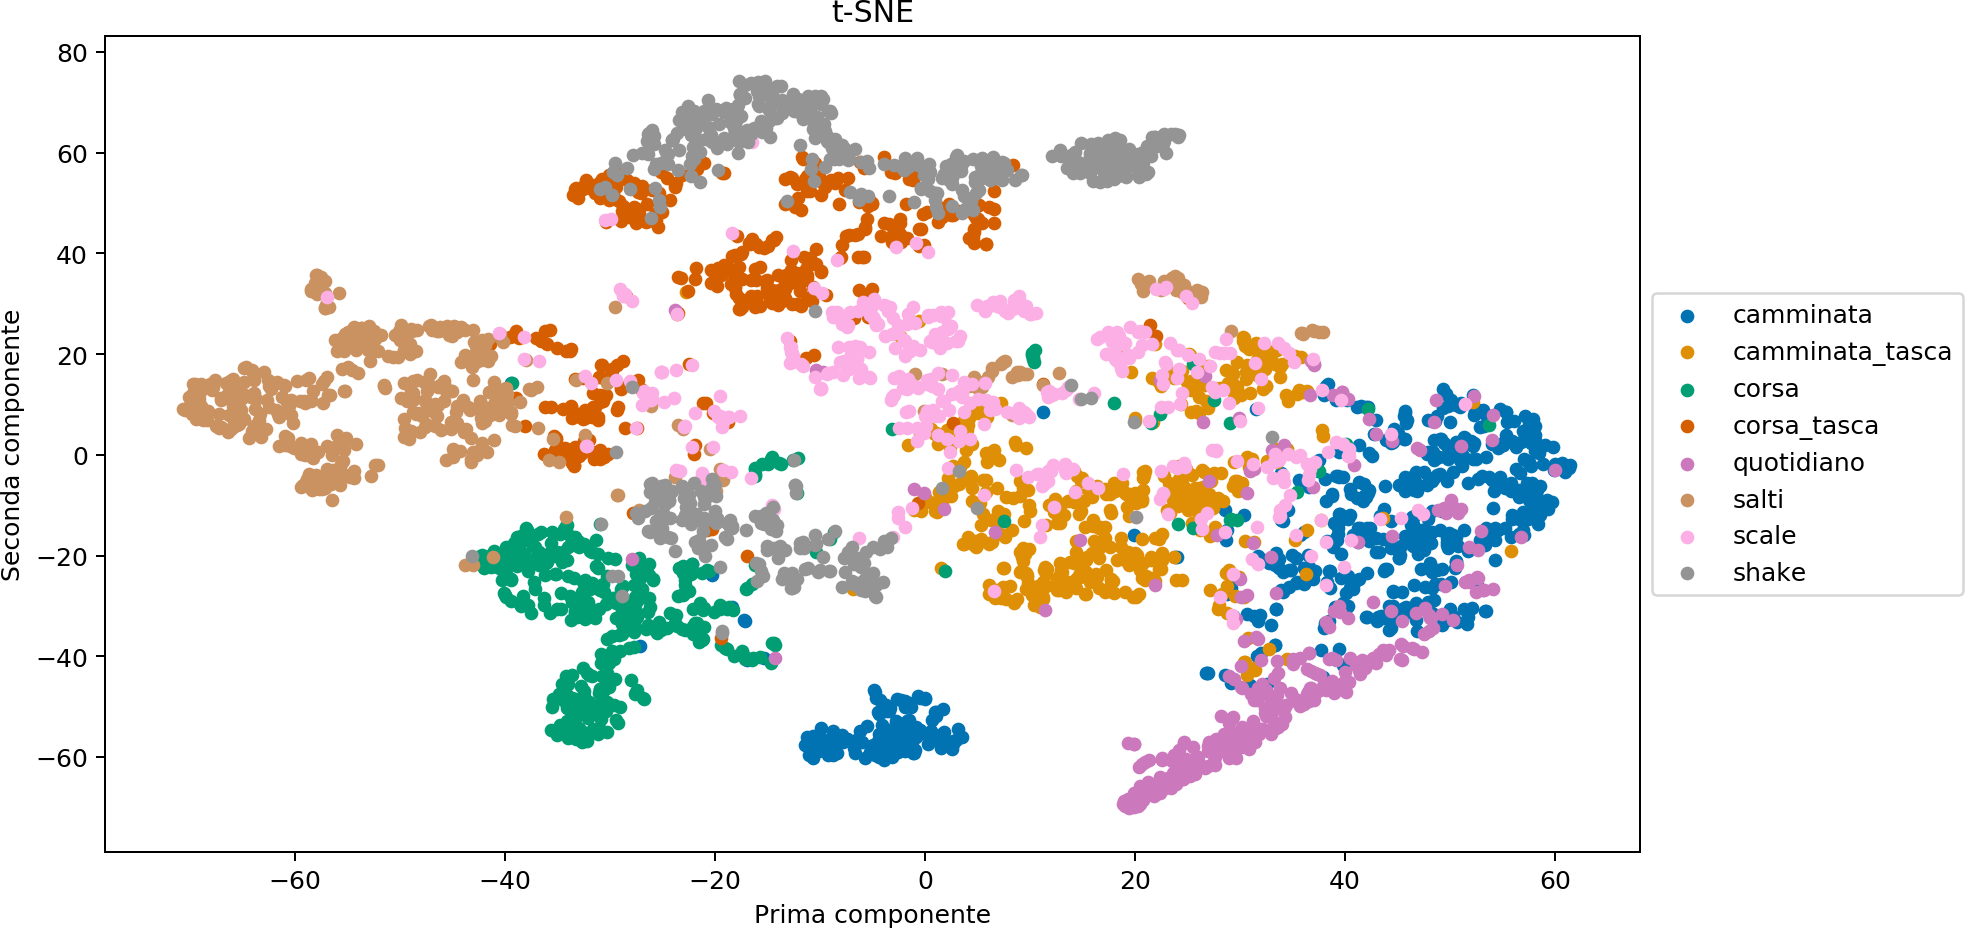
\includegraphics[width=\textwidth]{../figure/t-SNE.png}
\end{figure}
\end{frame}

\begin{frame}{I modelli}
I modelli per la classificazione analizzati sono: 
\begin{enumerate}
\item Analisi discriminante lineare
\item Analisi discriminante quadratica
\item Modello Multinomiale
\item Albero di Classificazione
\end{enumerate}

Per l'analisi il dataset è stato diviso in stima, convalida e verifica. 
\end{frame}

\begin{frame}{L'accuratezza dei modelli}
\begin{table}[H]
\centering
\caption{Accuratezza per i modelli adattati.}
\begin{tabular}{cc}
\toprule
       Modello &  Accuratezza \% \\
\midrule
 Multinomiale &          85.87 \\
           QDA &          85.87 \\
 Decision Tree &          82.94 \\
           LDA &          72.66 \\
\bottomrule
\end{tabular}
\label{tab:acc}
\end{table}
\end{frame}


\begin{frame}{Il modello}
\begin{figure}[H]
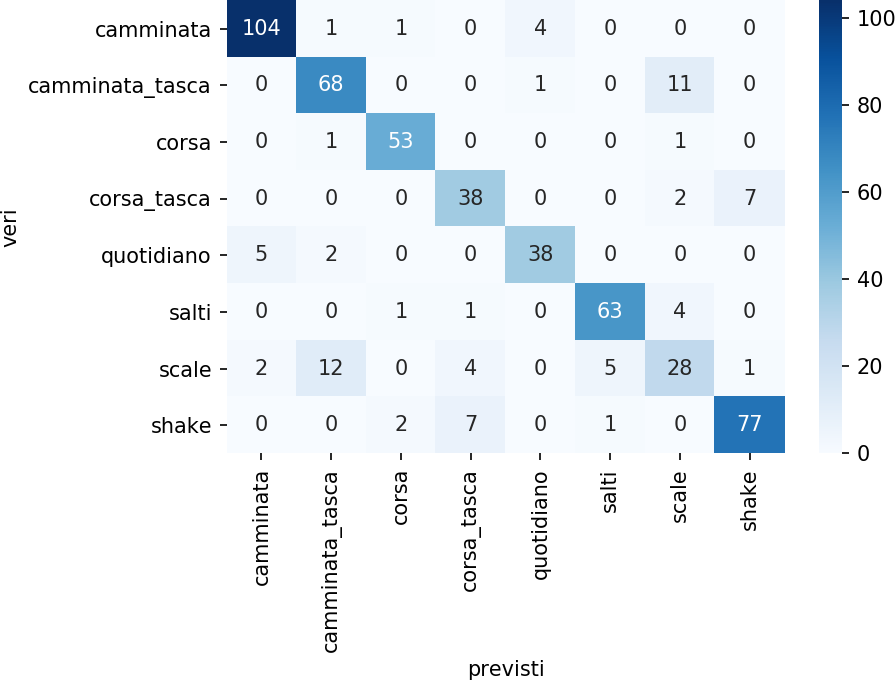
\includegraphics[width=0.8\textwidth]{../figure/confusionMatrix-Mn.png}
\end{figure}
\end{frame}

\begin{frame}{Importanza delle variabili}
\begin{figure}[H]
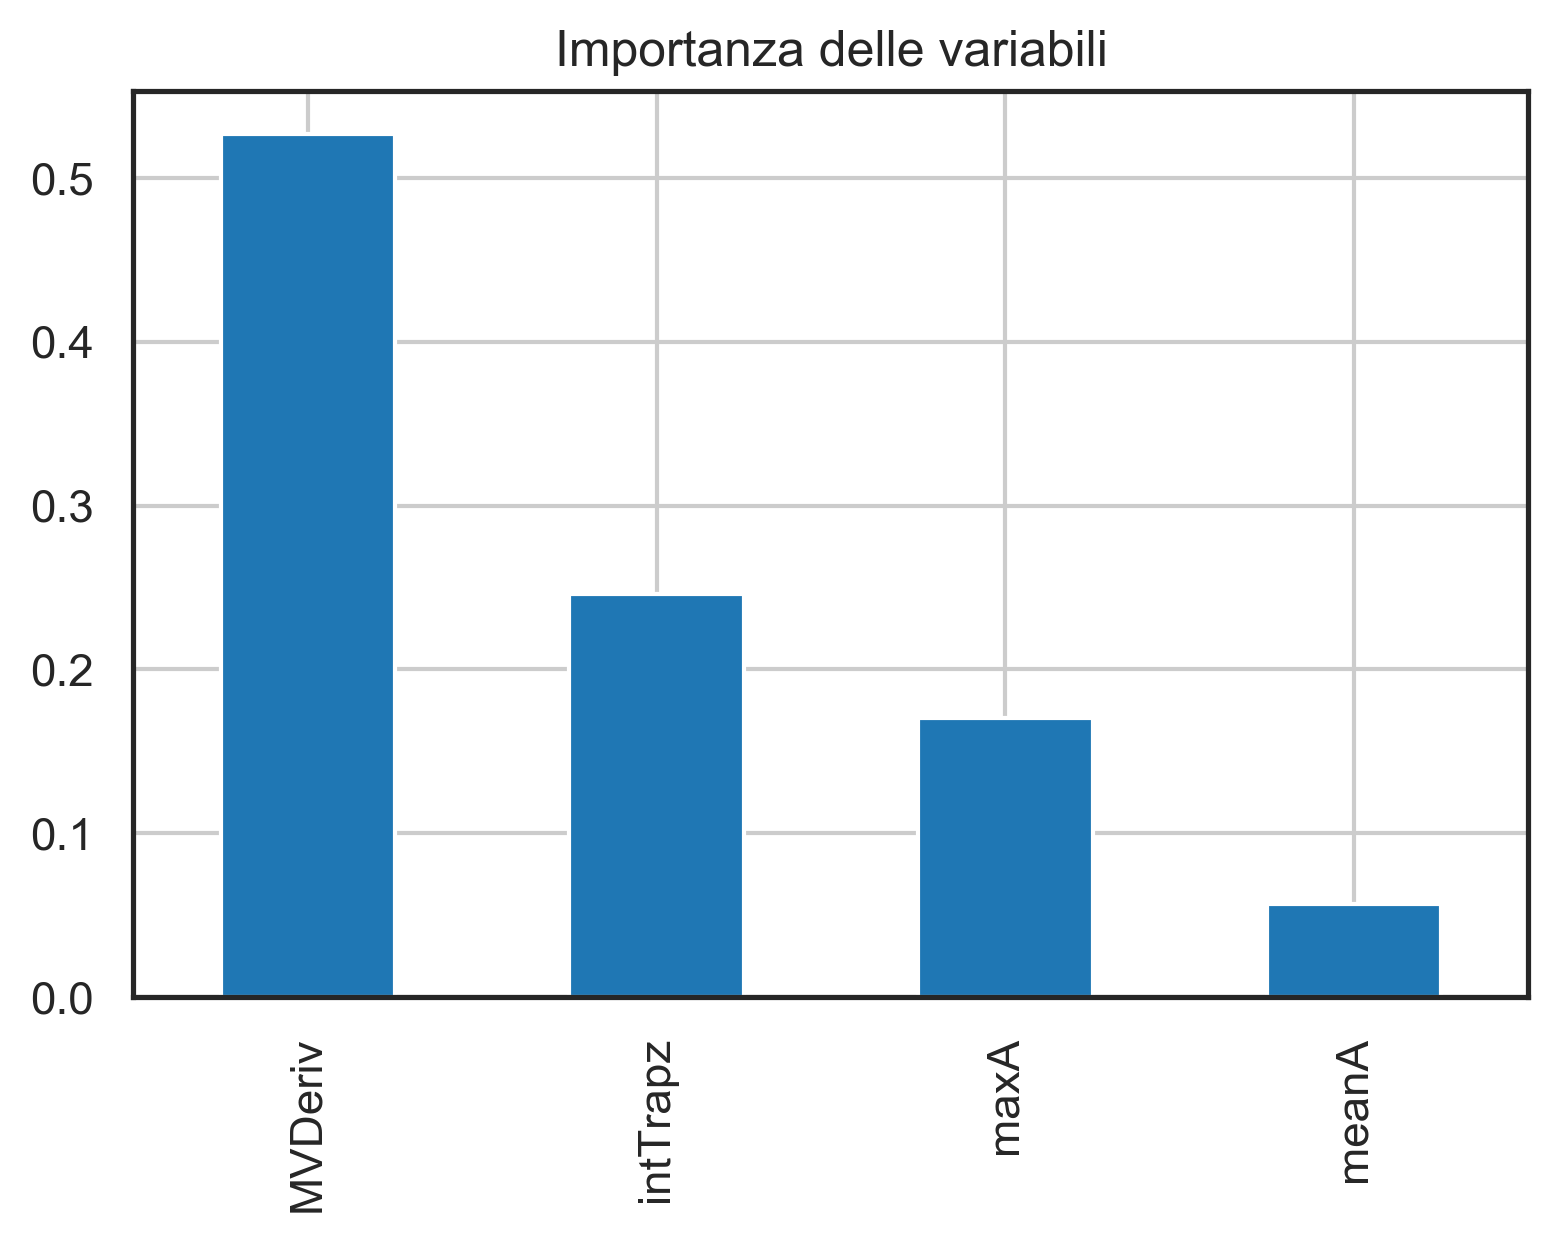
\includegraphics[width=0.8\textwidth]{../figure/importance-Tree.png}
\end{figure}
\end{frame}

\begin{frame}{Focus sul problema}
\textbf{OBIETTIVO}: evitare di confondere shake con altre attività.

\end{frame}

\begin{frame}{I modelli e lo shake}
\begin{table}[H]
\begin{tabular}{cc}
\toprule
Modello & Shake corretti \% \\
\midrule
Multinomiale & 90.59\\
QDA & 87.50\\
Albero decisionale ottimizzato & 83.53\\
Albero decisionale & 84.09\\
LDA & 80.30\\
\bottomrule
\end{tabular}
\end{table}

Per il problema in analisi, questi valori non sono sufficienti. 

Come fare?
\end{frame}

\begin{frame}{I pesi}
La percentuale di \emph{shake} correttamente classificati e l\rq{}accuratezza del modello variano in base al peso attribuito alla classe \emph{shake}.
\begin{figure}[H]
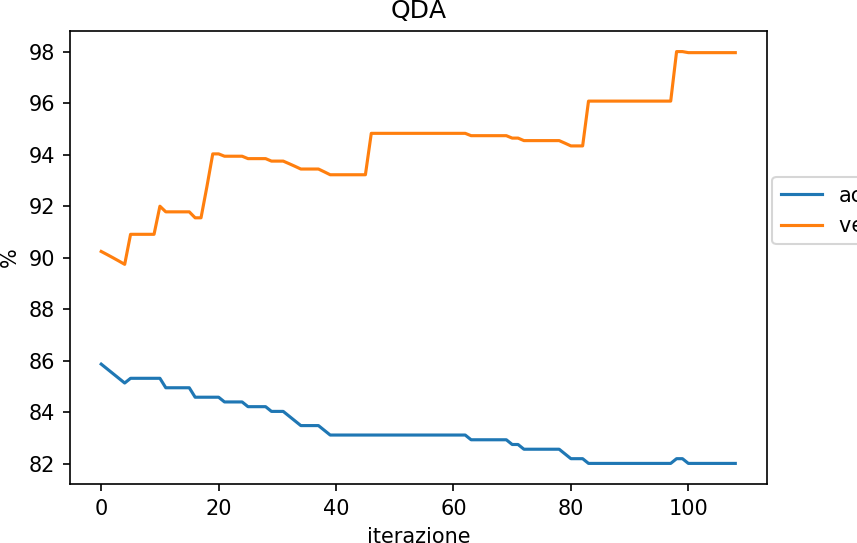
\includegraphics[width=\textwidth]{../figure/acc-vs-veripos-qda.png}
\end{figure}
\end{frame}

\begin{frame}{I pesi}
\textbf{Ma come scegliere i pesi?} \pause Ricerca sequenziale

\begin{figure}[H]
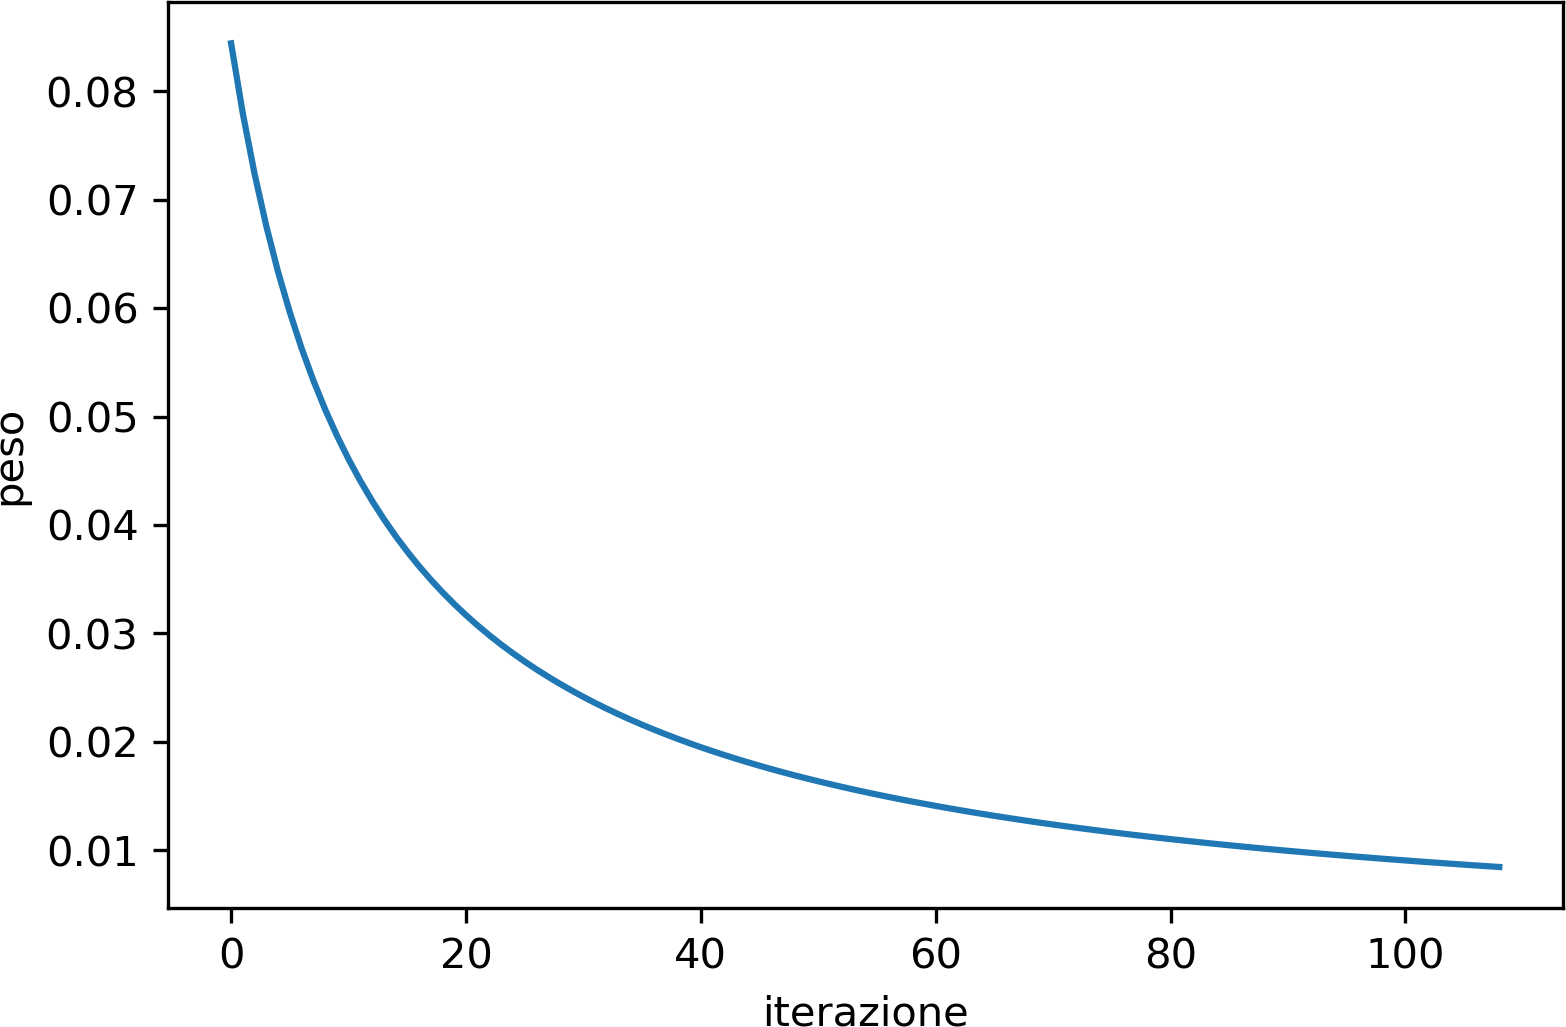
\includegraphics[width=0.6\textwidth]{../figure/andamento-pesi.png}
\end{figure}

\end{frame}

\begin{frame}{Il modello pesato}
È richiesto un tasso di {\em shake} correttamente classificati 
superiore al $98\%$.
\pause
\begin{table}[H]
\centering
\caption{Accuratezza per i modelli adattati sull'insieme di validazione.}
\begin{tabular}{cc}
\toprule
      Modello &  Accuratezza \% \\
\midrule
          QDA &          82.20 \\
 Multinomiale &          82.02 \\
          LDA &          68.62 \\
\bottomrule
\end{tabular}
\label{tab:acc_pen}
\end{table}
\end{frame}

\begin{frame}{Il modello pesato}
\begin{figure}[H]
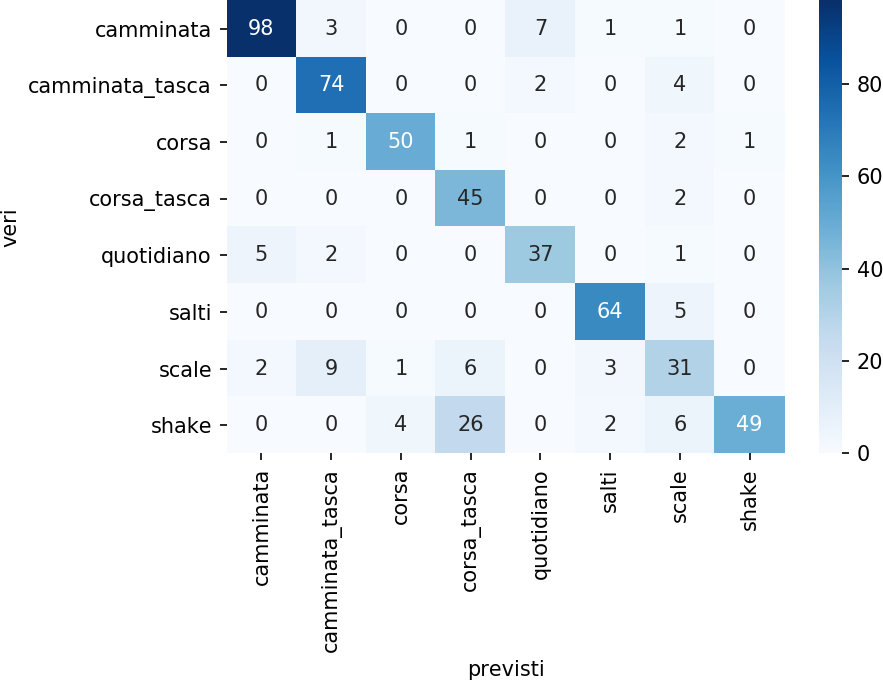
\includegraphics[width=0.8\textwidth]{../figure/confusionMatrix-QDA-penalizzata.png}
\end{figure}
\end{frame}

\begin{frame}{Sull'insieme di verifica}
\begin{columns}[T] % align columns
\begin{column}{.5\textwidth}
\begin{figure}[H]
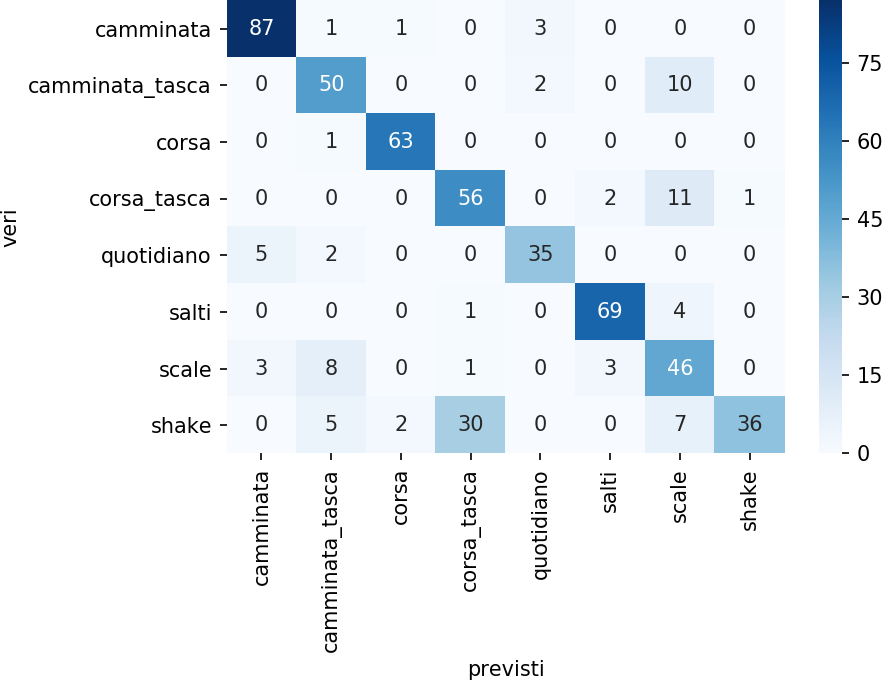
\includegraphics[width=\textwidth]{../figure/confusionMatrix-Mn-test.png}
\caption{Accuratezza 85.7\%, {\em shake} corretti 85.5\%.}
\end{figure}
\end{column}%
\hfill%
\begin{column}{.5\textwidth}
\begin{figure}[H]
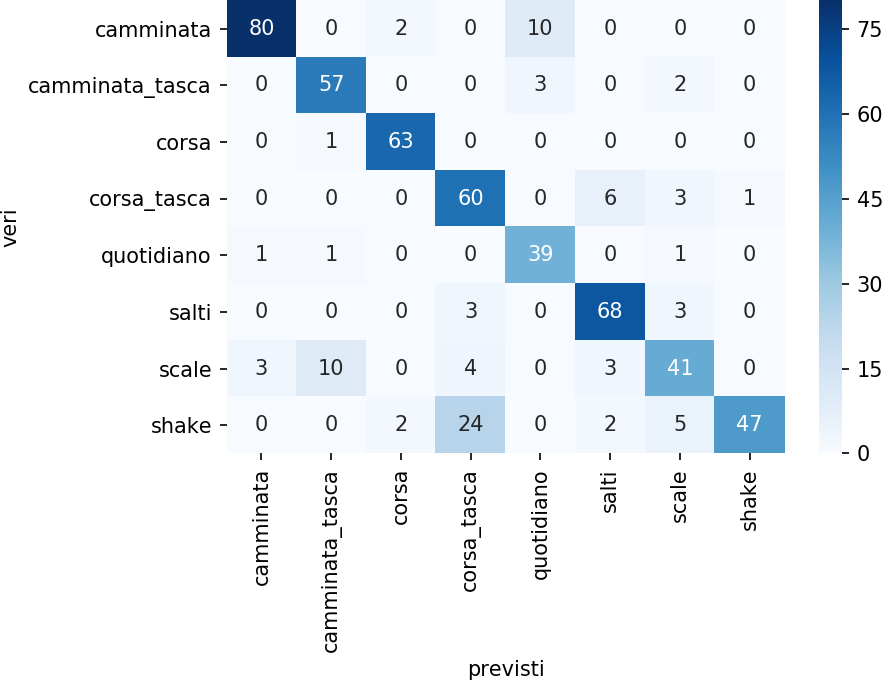
\includegraphics[width=\textwidth]{../figure/confusionMatrix-QDA-penalizzata-test.png}
\caption{Accuratezza 83.5\%, {\em shake} corretti 97.9\%.}
\end{figure}
\end{column}%
\end{columns}
\end{frame}

\section{Bibliografia}
\begin{frame}{Bibliografia}
\printbibliography
\end{frame}

\begin{frame}
\begin{figure}[H]

\includegraphics[width=\textwidth]{../figure/vodafone.png}
\end{figure}
\end{frame}
\end{document}
